\section{Data Science - Engineering}
\todo{Demonstrate the ability for analysis.}
\todo{Link to Related works - Not repeating. Might look at the sections and link them}

\todo{Section 1 is very interesting and further supports, or cast doubts or raises question marks about what is being said in the Related works.}
The process of collecting raw data from sources, transforming it so that it matches our system's requirements and loading it into a data-set is know as \textbf{ETL.} This \textit{acronym} represents \textit{Extract - Transform - Load.}

In this section, description regarding data pre-processing, model training, and model validations will be presented. Before the core analysis begins, it will be appropriate to talk about the dataset itself.


\begin{figure}[h!]
	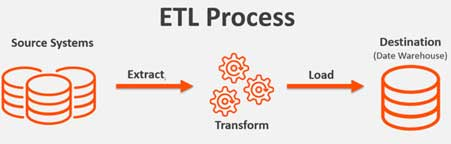
\includegraphics[width=\textwidth,height=\textheight,keepaspectratio]{fig/etl.jpg}
	\caption{Extract Transform Load.}
	\label{fig:ETL}
\end{figure}

Figure \ref{fig:ETL} shows the ETL process.

As mentioned in the previous section, the source of data for the purpose of this thesis was the Food and Agriculture Organization of the United Nations. To achieve my goals I focused on the \textbf{Value Of Agricultural Production} and in particular the \textbf{Gross Production Value.} This value was gotten by multiplying agricultural gross production by the output prices. In the data-sets used in this thesis paper, the gross production value is expressed in US dollars. This raw data set contains lots of columns which are not necessary. it's necessary to clean the data by dropping the unnecessary columns. 




\subsection{Data Extraction}

Different data sets are available separately. For the purpose of this thesis, I narrowed down on wheat. I adopted a consistent time-frame (\textbf{1965 to 2002}). The approach to this was: \textit{Given a set of features that are consistent with a particular agricultural product, the aim is to predict the Gross Production Value.}

To extract data, apart from the source, which has already been mentioned as the FAO, the format has to be considered. Data can be provided in various formats like a csv file, xml file, json object just to mention a few. the extracted Data for my work was in a csv file format. 

This work is focused on estimation of Gross-Production Value (GPV), indicative of GDP, based on wheat crop information of Hungary. The goal was to estimate GPV as the function of agri-land (Hectares) used for wheat, wheat quantity (Tons) produced and the crop yield (Hg/Ha Hectogram/Hectares). All four variables could not be found in a single data-set. They were found in four different data-sets, but from the single source.


\begin{figure}[h!]
	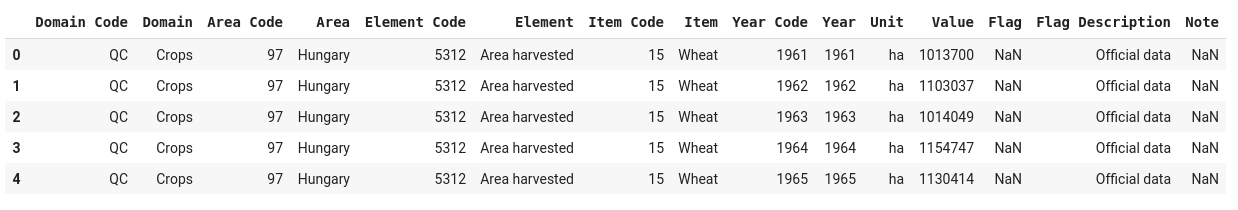
\includegraphics[width=\textwidth,height=\textheight,keepaspectratio]{fig/Area_Head.png}
	\caption{Raw Data Area.}
	\label{fig:Areaa_Head1}
\end{figure}

Figure \ref{fig:Areaa_Head1} shows the top 5 rows of the Wheat Area-harvested Data Set.

\begin{figure}[h!]
	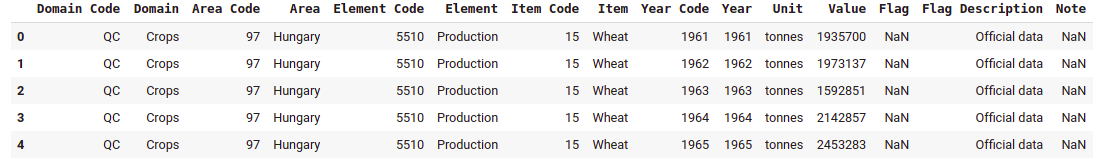
\includegraphics[width=\textwidth,height=\textheight,keepaspectratio]{fig/Quantity_Head.png}
	\caption{Raw Data Quantity.}
	\label{fig:Quantity_Head}
\end{figure}

Figure \ref{fig:Quantity_Head} shows the top 5 rows of the Quantity Data Set.



\begin{figure}[h!]
	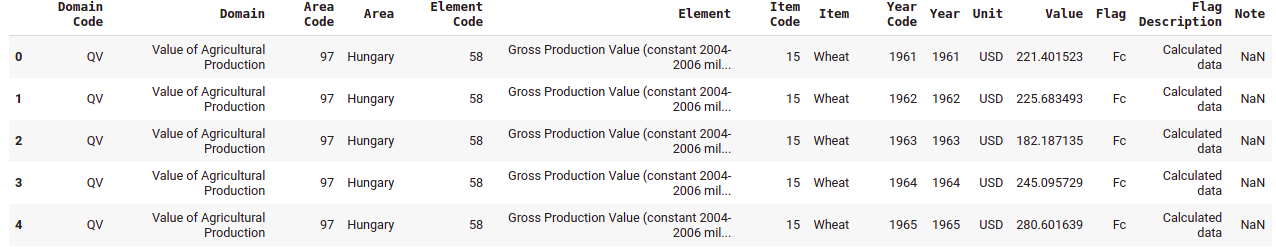
\includegraphics[width=\textwidth,height=\textheight,keepaspectratio]{fig/GPV_Head.png}
	\caption{Raw Data Gross Production Value.}
	\label{fig:GPV_Head}
\end{figure}

Figure \ref{fig:GPV_Head} shows the top 5 rows of the Gross Production Value Data Set.


The correlation strength between the variables of the system is shown in the Figure below. Light and yellow colors indicate a strong correlation, while deeper colors show weak relationship. The weakest correlation can be observed between agricultural area and the yield, although it looks illogical. This is because of the unique definition of yield performance. So, it can be said that they are independent from one another. Similarly, weaker correlation can be observed amongst area, wheat quantity and GPV. It can be concluded that they will affect each other less, but they cannot be termed as independent parameters.  

Finally, the most valuable observation from Figure~\ref{fig:Corr} is that GPV is a strong function of quantity, yield and area (in ascending order from the quantity variable to area). So, inclusion/exclusion of these variables will severely affect the accuracy. Although there are inter-dependencies, but such dependencies can be better taken care of by the proposed solution.


\begin{figure}[h!]
	\centering
	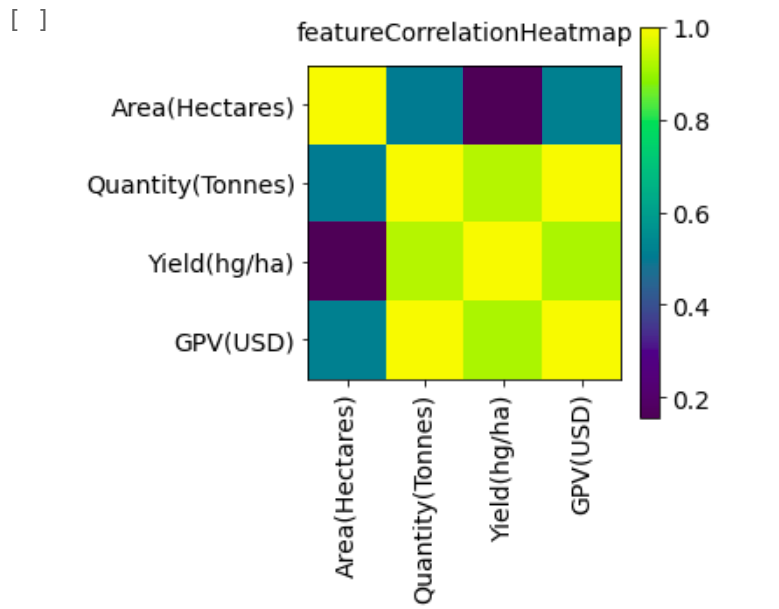
\includegraphics[width=0.35\textwidth]{fig/correlation.png}
	\caption{Feature Correlation Heatmap}
	\label{fig:Corr}
\end{figure}


 




\subsection{Data Transformation} 

This is the data-validation step. The guiding principle is: 

\textquote{The garbage in, garbage out (GIGO) is the concept that flawed, or nonsense input data produces nonsense output or garbage.}



The pertinent data-sets contained too much extra and irrelevant information as well some null columns. Using Pandas, the data-sets were cleaned, irrelevant columns were dropped and desired variables were collected into one data-set a tabular frame using the year as the index. A glimpse of the data-frame is shown below:



\begin{figure}[h!]
	\centering
	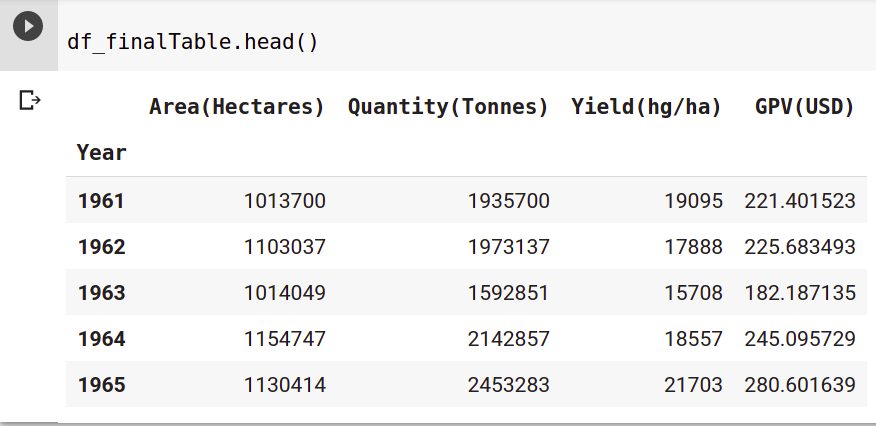
\includegraphics[width=0.4\textwidth,height=\textheight,keepaspectratio]{fig/finaltable.png}
	\caption{Concatenated Final Dataset}
	\label{fig:CFD}
\end{figure}


To make the downloaded data set globally available, I uploaded it to my GitHub repository.\cite{adeyemo_2020}

\begin{lstlisting}[language=Python]
	url_wheatArea = 'https://raw.githubusercontent.com/k-plasma/Machine-Learning-Models-for
	-Agricultural-Data-Applications/master/wheatArea.csv'	
	
	url_wheatGrossProduction = 'https://raw.githubusercontent.com/k-plasma/Machine-Learning-Models-for
	-Agricultural-Data-Applications/master/wheatGrossProductionValue.csv'	
	
	url_wheatProductionQuantity = 'https://raw.githubusercontent.com/k-plasma/Machine-Learning-Models-for
	-Agricultural-Data-Applications/master/wheatProductionQuantity.csv'	
	
	url_wheatYield = 'https://raw.githubusercontent.com/k-plasma/Machine-Learning-Models-for
	-Agricultural-Data-Applications/master/wheatYield.csv'
\end{lstlisting}




Each set of data set contained lots of columns which are repetitive and irrelevant to the task at hand. These columns include: \textit{"Domain Code","Domain",
	"Area Code","Area","Element Code","Element","Item Code","Item",
	"Year Code","Unit","Flag","Flag Description","Note"}


The repetitive columns constitute noise which isn't required. I dropped these to narrow down on the vital data necessary for my task. Two columns are left: \textit{"Year", "Value".} Since the word \textit{"Value"} appears in the different data-sets, it's renamed here as \textit{"Area(Hectares)"} to clearly indicate that this value refers to the measurement of the area.


\begin{lstlisting}[language=Python]
	df_wheatArea.drop(columns=["Domain Code","Domain",
	"Area Code","Area","Element Code","Element","Item Code","Item",
	"Year Code","Unit","Flag","Flag Description","Note"], axis=1, inplace=True)
	
	df_wheatArea.columns = ['Year', 'Area(Hectares)'] 
	
	df_wheatArea.head()
\end{lstlisting}

A similar transformation is performed on the other data-sets. The resulting individual data-sets are displayed in Fig \ref{fig:heads} : 
\begin{figure}
	\centering
	\begin{subfigure}{.25\textwidth}
		\centering
		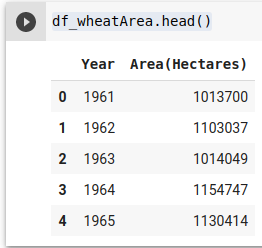
\includegraphics[width=.4\linewidth]{fig/areaHectares.png}
		\caption{Area}
		\label{fig:sub1}
	\end{subfigure}%
	\begin{subfigure}{.24\textwidth}
		\centering
		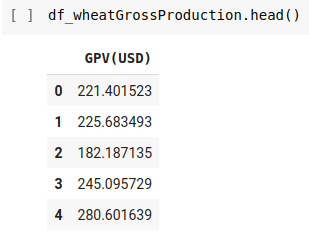
\includegraphics[width=.4\linewidth]{fig/gpv.png}
		\caption{G.P.V}
		\label{fig:sub2}
	\end{subfigure}
	\begin{subfigure}{.25\textwidth}
		\centering
		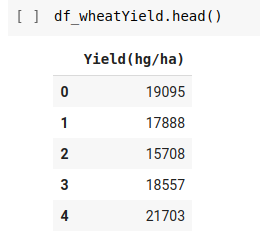
\includegraphics[width=.4\linewidth]{fig/yield.png}
		\caption{Yield}
		\label{fig:sub3}
	\end{subfigure}
	\begin{subfigure}{.24\textwidth}
		\centering
		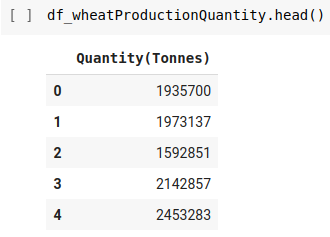
\includegraphics[width=.4\linewidth]{fig/quantityTonnes.png}
		\caption{Quantity}
		\label{fig:sub4}
	\end{subfigure}

	\caption{Individual Transformed Data-Sets}
	\label{fig:heads}
\end{figure}



\section{Data Loading}

This is about loading the data to the database. Databases can be divided into either Relational or non-relational databases. Relational database store data in tables and rows. Non relation store data in JSON object. For the purpose of my work, the Python Pandas data-frame was used. This is a two-dimensional data structure where the data is aligned in rows and columns. The data can then be manipulated and vital information extracted.

\begin{figure}[h!]
	\centering
	
\includegraphics[width=0.35\textwidth]{fig/panda.png}
	\caption{Pandas DataFrame}
	\label{fig:panda}
\end{figure}


\section{Recurring Neural Network}
\begin{figure}[h!]
	\centering
	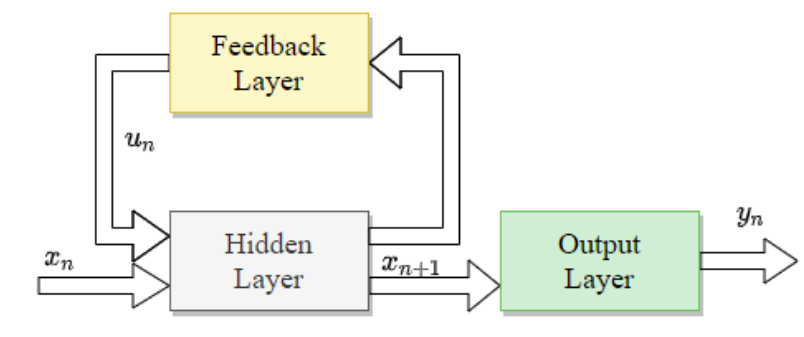
\includegraphics[width=0.35\textwidth]{fig/rnn.png}
	\caption{Recurrent Neural Network (RNN)}
	\label{fig:rnn}
\end{figure}
A representative RNN is shown in Figure ~\ref{fig:rnn} showing the hidden layer. The updating of the weight is accomplished as the function of current inputs and previous outputs. Usually, the weights are updated on the basis of output gradients. The weights are only updated, if the underlying gradients are non-zero. As the learning goes on, gradients begin to vanish. At sometimes the gradients are zero, but they should not be. In deep learning literature, this phenomenon is termed as gradient-vanishing problem - GVP \cite{haykin2009neural}. To avoid GVP, two variants of RNNs have been proposed. LSTM (Long-Short Term Memory) recurrent neural network and GRU (Gated-Recurrent Unit).

\subsubsection{LSTM-RNN}

The problem of GVP can be solved in two ways, firstly using long-term and short-term memories and secondly using the first way in gated fashion. The first method is termed as long-term short-term memory. The short-term serves usually as RNN works, while long-term memory serves to keep the most relevant and updated information. Although, this method is computationally costly, it effectively overcomes the issue of vanishing gradients. 

A LSTM has a comparable control stream as a repetitive neural organization. It measures information passing on data as it engenders forward. The distinctions are the activities inside the LSTM's cells. These tasks are utilized to permit the LSTM to keep or fail to remember data. 

The central idea of LSTM is the cell state and its different doors. The cell state goes about as a vehicle thruway that moves relative data right down the grouping chain. You can consider it the "memory" of the organization. The cell state, in principle, can convey important data all through the handling of the grouping. So even data from the prior time steps can advance toward later time steps, decreasing the impacts of momentary memory. As the cell state goes on its excursion, data gets added or eliminated to the cell state by means of entryways. The entryways are diverse neural organizations that choose which data is permitted on the cell state. The doors can realize what data is pertinent to keep or fail to remember during preparing. 


\subsubsection{GRU}

The Gated Recurrent Unit (GRU) can be seen as an improvement of the LSTM, which does not utilize unequivocal cell states. Another distinction is that the LSTM straightforwardly controls the measure of data changed in the hidden state utilizing separate response and forgetting gateways. Then again, a GRU utilizes a solitary reset entryway to accomplish a similar objective. Be that as it may, the fundamental thought in the GRU is similar to that of a LSTM, regarding how it somewhat resets the hidden states. 

The GRU is the fresher age of Recurrent Neural organizations and is quite like a LSTM. GRU utilizes the hidden state to move data. It likewise just has two entryways, a reset door and update door. The update door acts like the fail to remember and enter the entryway of a LSTM. It chooses what data to discard and what new data to add.  

The reset door is another entryway. It is utilized to choose how much past data not to remember. Furthermore, GRU has less tensor activities; accordingly, they are somewhat speedier to prepare than LSTMs. There is definitely not an unmistakable fact as to which one is better. Scientists and designers typically attempt both to figure out which one turns out better for their utilization case.  

To summarize, RNNs are useful for handling arrangement information for forecasts however they experience momentary memory. LSTM and GRU were made as a strategy to alleviate momentary memory utilizing components called gateways. Gates are simply neural organizations that control the progression of data coursing through the arrangement chain. LSTM and GRU are utilized in best-in-class profound learning applications like discourse acknowledgment, discourse amalgamation, common language understanding, and so on. 

\subsubsection{Topology}

In this work, LSTM and GRU variants of recurrent networks have been used as computational machines. The results of these algorithms are compared with a feed-forward network. For all the networks the number of input neurons are three, with 64 hidden neurons and a single output neuron.  

In the feedforward network, 64 neurons are divided equally in 8 consecutive hidden layers. Although the network has become extremely complex, but the complexity remains essentially in vain. The training accuracy and prediction value were found to be poor. 

The structure of LSTM requires that some neurons be assigned to the memory making region, known as cell, which serves the purpose of holding long-term desired information. The training machines can assign different number of neurons to cell memory and to the hidden layer depending upon the user's choice. The decision, taken by the user are dictated by various factors. Larger amount of memory can improve accuracy of prediction hugely, but speed of consecutive predictive operations could be impeded. So, the decision should be taken based on the optimum between speed and accuracy. 

GRU does not require dedicated long-term memory, but it inherits the features of LSTM. It does update the neurons and lets them forget older data in similar fashion to that of LSTM. This algorithm can provide better speed and accuracy management.  

A representative Feed Forward Network is shown in Figure ~\ref{fig:feedforward} showing the resulting graph.

We can conclude that this method will not serve our purpose. 


\begin{figure}[h!]
	\centering
	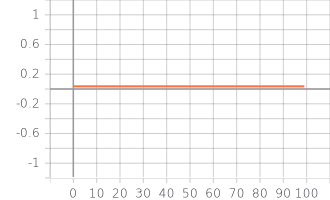
\includegraphics[width=0.35\textwidth]{fig/epoch_accuracy.png}
	\caption{Feed Forward Network}
	\label{fig:feedforward}
\end{figure}



\subsubsection{Model Training}

The models have been trained with extensive number of epochs. The training performance and achieved accuracy are shown in Figure ~\ref{fig:feedforward} and Figure ~\ref{fig:trg} respectively. The x-axis indicates the epoch number, while the y-axis indicates the training loss. From Figure ~\ref{fig:feedforward}, it should be noticed that even with 100 epochs, the performance of feed-forward network could not be improved. So, further analysis of this network is left out. Figure ~\ref{fig:train} indicates the training performance of the proposed RNN’s networks. As the training continues epoch-by-epoch, networks keep on learning the underlying system better and better. So, LSTM indicates some fluctuations, but they can be ignored in comparison to feedforward network. It can clearly be seen that accuracy of LSTM and GRU has surpassed that of feed-forward network. This might have occurred due to foundations of LSTM and GRU on recurrent networks. 

\begin{figure}[h!]
	\centering
	\begin{subfigure}{.5\textwidth}
		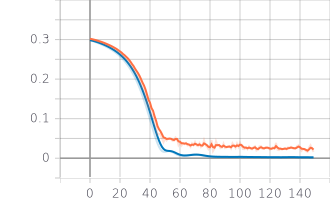
\includegraphics[width=0.35\textwidth]{fig/trg.png}
		\caption{LSTM vs GRU I}
		\label{fig:trg}
	\end{subfigure}%
	\begin{subfigure}{.5\textwidth}
			\centering
		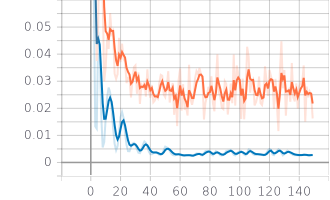
\includegraphics[width=0.35\textwidth]{fig/train.png}
		\caption{LSTM vs GRU II}
		\label{fig:train}
	\end{subfigure}	
	\caption{Training Performance between LSTM and GRU}
\end{figure}